%! Author = Omar Iskandarani
%! Title = Long-Distance Swirl Gravity from Chiral Swirling Knots with Central Holes
%! Date = Sept 25, 2025
%! Affiliation = Independent Researcher, Groningen, The Netherlands
%! License = © 2025 Omar Iskandarani. All rights reserved. This manuscript is made available for academic reading and citation only. No republication, redistribution, or derivative works are permitted without explicit written permission from the author. Contact: info@omariskandarani.com
%! ORCID = 0009-0006-1686-3961
%! DOI = 10.5281/zenodo.17155854

\newcommand{\paperversion}{\textbf{v0.0.2}} % Semantic versioning: vMAJOR.MINOR.PATCH
\newcommand{\papertitle}{Long-Distance Swirl Gravity from Chiral Swirling Knots with Central Holes}
\newcommand{\paperdoi}{10.5281/zenodo.17204124}

%========================================================================================
% PACKAGES AND DOCUMENT CONFIGURATION
%========================================================================================
\documentclass[reprint,aps,onecolumn,nofootinbib]{revtex4-2}

% ====== minimal packages ======
\usepackage{amsmath,amssymb,amsfonts}
\usepackage{bm}
\usepackage{physics}
\usepackage{microtype}
\usepackage{tcolorbox}
\usepackage{hyperref}
\hypersetup{colorlinks=true,linkcolor=blue,citecolor=blue,urlcolor=blue}

% ==== Packages ====
\usepackage[T1]{fontenc}
\usepackage{lmodern}
\usepackage{booktabs}
\usepackage[utf8]{inputenc}
\usepackage[caption=false]{subfig}

% ===== Gauge sector macros =====
\renewcommand{\Tr}{\mathrm{Tr}}
\newcommand{\ii}{\mathrm{i}}
\newcommand{\GsA}{G^a_{\mu\nu}}
\newcommand{\WsI}{W^i_{\mu\nu}}
\newcommand{\Bmn}{B_{\mu\nu}}

% ===============================
% Macros (canonicalized)
% ===============================

% swirl arrows (context-aware)
\newcommand{\swirlarrow}{%
    \mathchoice{\mkern-2mu\scriptstyle\boldsymbol{\circlearrowleft}}%
    {\mkern-2mu\scriptstyle\boldsymbol{\circlearrowleft}}%
    {\mkern-2mu\scriptscriptstyle\boldsymbol{\circlearrowleft}}%
    {\mkern-2mu\scriptscriptstyle\boldsymbol{\circlearrowleft}}%
}
\newcommand{\swirlarrowcw}{%
    \mathchoice{\mkern-2mu\scriptstyle\boldsymbol{\circlearrowright}}%
    {\mkern-2mu\scriptstyle\boldsymbol{\circlearrowright}}%
    {\mkern-2mu\scriptscriptstyle\boldsymbol{\circlearrowright}}%
    {\mkern-2mu\scriptscriptstyle\boldsymbol{\circlearrowright}}%
}

% Canonical symbols
\newcommand{\vswirl}{\mathbf{v}_{\swirlarrow}}
\newcommand{\vswirlcw}{\mathbf{v}_{\swirlarrowcw}}
\newcommand{\SwirlClock}{S_{(t)}^{\swirlarrow}}
\newcommand{\SwirlClockcw}{S_{(t)}^{\swirlarrowcw}}
\newcommand{\omegas}{\boldsymbol{\omega}_{\swirlarrow}}  % swirl vorticity
\newcommand{\vscore}{v_{\swirlarrow}}                    % shorthand: |v_swirl| at r=r_c
\newcommand{\vnorm}{\lVert \vswirl \rVert}               % swirl speed magnitude
\newcommand{\rhof}{\rho_{\!f}}                           % effective fluid density
\newcommand{\rhoE}{\rho_{\!E}}                           % swirl energy density
\newcommand{\rhom}{\rho_{\!m}}                           % mass-equivalent density
\newcommand{\rc}{r_c}                                    % string core radius (swirl string radius)
\newcommand{\FmaxEM}{F_{\mathrm{EM}}^{\max}}             % EM-like maximal force scale
\newcommand{\FmaxG}{F_{\mathrm{G}}^{\max}}               % G-like maximal force scale
\newcommand{\Lam}{\Lambda}                               % Swirl Coulomb constant
\newcommand{\Om}{\Omega_{\swirlarrow}}                   % swirl angular frequency profile
\newcommand{\alpg}{\alpha_g}                             % gravitational fine-structure analogue
% --- Minimal macro prelude (safe, local) ---
\providecommand{\rc}{r_c}
\newcommand{\omegaVec}{\boldsymbol{\omega}}
\newcommand{\rhoF}{\rho_{\!f}}     % effective fluid density
\newcommand{\rhoM}{\rho_{\!m}}     % mass-equivalent density
\newcommand{\OmegaCore}{\Omega_{\mathrm{core}}}
\newcommand{\bg}{\mathrm{bg}}
\newcommand{\core}{\mathrm{core}}
\newcommand{\GammaC}{\Gamma_C}

% ===============================
% Policy: the golden constant is only allowed via hyperbolic functions.
\newcommand{\xig}{\operatorname{asinh}\!\left(\tfrac{1}{2}\right)}
\newcommand{\phig}{\exp(\xig)}
\newcommand{\phialg}{\bigl(1+\sqrt{5}\bigr)/2}
\newcommand{\xigold}{\tfrac{3}{2}\,\xig}
\newcommand{\GoldenDeclare}{%
    \textbf{Golden (hyperbolic)}:\ \(\ln\phi=\xig\), hence \(\phi=\phig\).
    \ \emph{(Equivalently, \(\phi=\phialg\); the algebraic form is derivative.)}%
}
\usepackage{graphicx}
\usepackage{geometry}
\geometry{margin=1in}

\usepackage{tikz}
\usetikzlibrary{calc,arrows.meta,decorations.markings,decorations.pathmorphing,knots,hobby,intersections.pathreplacing,shapes.geometric,spath3}

% A tiny style for loop arrows
\tikzset{
    looparrow/.style={-{Stealth[length=2.5mm,width=1.8mm]},thick},
    knotline/.style={ultra thick, blue!70},
    testloopON/.style={thick, draw=green!60!black},
    testloopOFF/.style={thick, draw=red!70},
    axes/.style={very thick, black},
}

\usepackage{siunitx}
\AtBeginDocument{\RenewCommandCopy\qty\SI}

% Styling helpers
\tikzset{
    axisline/.style={very thick, black},
    corecircle/.style={thick, dashed, gray},
    knotline/.style={ultra thick, blue!65},
    swirlarrow/.style={-{Stealth[length=3mm,width=2mm]}, thick},
    vline/.style={-{Stealth[length=3mm,width=2mm]}, thick, teal!70!black},
    tube/.style={line width=6pt, line cap=round},
    ghost/.style={opacity=0.25},
    labelbox/.style={fill=white, inner sep=2pt, rounded corners=2pt},
}


% ------- Shared styles  -------
\tikzset{
    knot diagram/every strand/.append style={
        line cap=round,
        line join=round,
        ultra thick,
        red
    },
    every knot/.style={line cap=round,line join=round,very thick},
    strand/.style={line cap=round,line join=round,line width=3pt,draw=black},
    over/.style={preaction={draw=white,line width=6.5pt}},
}


\begin{document}
    \title{\papertitle }
    \author{Omar Iskandarani}
    \affiliation{Independent Researcher, Groningen, The Netherlands}
    \thanks{ORCID: 0009-0006-1686-3961,\\
            DOI: \paperdoi \\
            Version: \paperversion \\
    \textbf{Keywords:} Swirl-String Theory, Topological Gravity, Entropic Force, Circulation Quantization, Flat-Space Field Theory
    }
    \date{\today}

    \begin{abstract}
    We derive long-range gravitational attraction in Swirl--String Theory (SST) as a direct consequence of \emph{chiral swirling knots}---topological vortex filaments such as the trefoil (\(3_1\)), cinquefoil (\(5_1\)), (\(5_2\)), and stevedore (\(6_1\)).
    Each knot encloses a central rotational line, which acts as an anchor of circulation.
    Using Cauchy's integral theorem, we show that the circulation measured around any loop enclosing this axis is quantized by the knot's winding number.
    This quantization is expressed by the Swirl Clock \(\SwirlClock\), and its persistence explains why neutral molecules (e.g.\ H\(_2\) attract in otherwise flat space: their knots are connected via the same central swirl line extending beyond the equal-pressure boundary.
    \end{abstract}


    \maketitle


\section{Chiral Swirling Knots and Central Holes}
    Consider a chiral knot $K$ embedded in $\mathbb{R}^3$, such as~\ref{fig:knot-gallery}:

    \begin{figure}[htbp]
        \centering
        \subfloat[$3_1$ (trefoil)\label{fig:3-1}]{
            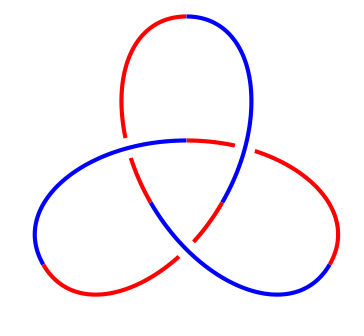
\includegraphics[width=0.22\linewidth]{3_1}}
        \hfill
        \subfloat[$5_1$ (cinquefoil)\label{fig:5-1}]{
            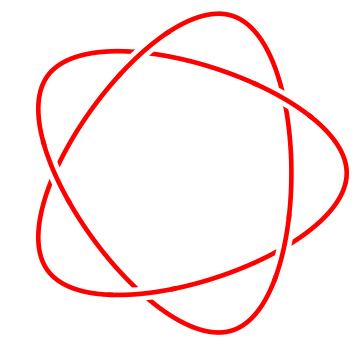
\includegraphics[width=0.22\linewidth]{5_1}}
        \hfill
        \subfloat[$5_2$ (cinquefoil twist)\label{fig:5-2}]{
            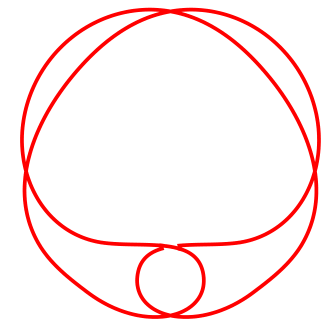
\includegraphics[width=0.22\linewidth]{5_2}}
        \hfill
        \subfloat[$6_1$ (stevedore)\label{fig:6-1}]{
            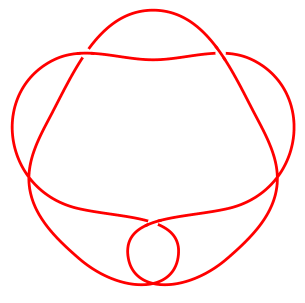
\includegraphics[width=0.22\linewidth]{6_1}}
        \caption{Canonical knot gallery.}
        \label{fig:knot-gallery}
    \end{figure}

    Each knot can be parametrized on a torus with major radius $R$ and minor radius $r$.
    The core tube of radius $r_c$ supports a tangential swirl velocity $\vswirl$, defining the \emph{Swirl Clock} $\SwirlClock$.

    A defining feature is that all these knots possess a \emph{central hole} threaded by a straight axis (taken as the $z$-axis).
    This axis is the ``fabric line'' of flat space: it is the singularity in the analytic swirl potential.


    \begin{figure}[t]
        \centering
        \begin{tikzpicture}[scale=1.0,>=Latex]
            \foreach \y in {0,0.9,1.8,2.7}{
                \draw[rounded corners=8pt,thick] (-3,\y) -- (3,\y) -- (2.5,\y+0.5) -- (-3.5,\y+0.5) -- cycle;
                \node[gray] at (3.4,\y+0.25) {$\Sigma_{t}$};
            }
            \draw[->,very thick,blue] (0,-0.2) -- (0,3.4) node[right] {$u^\mu \parallel \partial^\mu T$};
            \draw[->,thick] (-1.3,1.3) -- (-0.5,1.3) node[above] {$h^\mu{}_\nu$};
        \end{tikzpicture}
        \caption{Preferred foliation by the clock field $T(x)$ with unit timelike $u^\mu$, and spatial projector $h_{\mu\nu}=g_{\mu\nu}+u_\mu u_\nu$.}\label{fig:foiliation}
    \end{figure}


    % ============================
    % Figure: Trefoil + central axis + circulation loops (clean, layered)
    % ============================
    \begin{figure}[htbp]
        \centering
        \begin{tikzpicture}[scale=0.90, line cap=round, line join=round]
            % ------------------------
            % Parameters
            % ------------------------
            \def\R{3.20}      % major radius (to center of tube)
            \def\rtube{0.95}  % tube radius (for planar projection amplitude)
            \def\Rin{\R-\rtube}
            \def\Rout{\R+\rtube}

            % ------------------------
            % Styles
            % ------------------------
            \tikzset{
                axisline/.style={->, line width=0.6pt, black!70},
                annulusfill/.style={fill=gray!10, even odd rule},
                annulusline/.style={draw=gray!55, line width=0.6pt},
                corecircle/.style={draw=black!70, line width=0.8pt},
                outercircle/.style={draw=black!60, line width=0.8pt, dash pattern=on 3pt off 2pt},
                labelbox/.style={fill=white, draw=black!20, rounded corners=2pt, inner sep=3pt},
                knotunder/.style={draw=blue!45!black, line width=1.4pt},
                knotover/.style={
                    draw=blue!80!black, line width=1.4pt,
                    preaction={draw=white, line width=3.2pt, line cap=round}
                },
                knotarrows/.style={
                    postaction={decorate},
                    decoration={
                        markings,
                        mark=at position 0.18 with {\arrow{Latex}},
                        mark=at position 0.52 with {\arrow{Latex}},
                        mark=at position 0.86 with {\arrow{Latex}}
                    }
                }
            }

            % ------------------------
            % Axes (x-y plane view)
            % ------------------------
            \draw[axisline] (-0.3,0) -- (6.8,0) node[below right] {$x$};
            \draw[axisline] (0,-3.6) -- (0,3.6) node[left] {$y$};

            % Central rotational axis marker (z comes out of plane at origin)
            \fill[black] (0,0) circle(2pt);
            \node[below left] at (0,0) {\small central axis ($z$)};

            % ------------------------
            % Torus annulus (projection band)
            % ------------------------
            \fill[annulusfill] (0,0) circle (\Rout) (0,0) circle (\Rin);
            \draw[annulusline] (0,0) circle (\Rin);
            \draw[annulusline] (0,0) circle (\Rout);
            \node[labelbox, align=left] at (\R,-2.35) {\footnotesize torus annulus $[R-\!r,\,R+\!r]$};

            % ------------------------
            % Circulation test loops in z=0 plane
            % ------------------------
            \foreach \RR in {2.10, 2.60, 3.20} {
                \draw[corecircle] (0,0) circle (\RR);
            }
            \node[labelbox] at (2.10, 1.25) {\(\Gamma \approx -3\,\kappa\)};
            \node[labelbox] at (2.60,-1.25) {\(\Gamma \approx -3\,\kappa\)};
            \node[labelbox] at (3.20, 1.25) {\(\Gamma \approx -3\,\kappa\)};

            \draw[outercircle] (0,0) circle (4.6);
            \node[labelbox] at (4.6,-1.25) {\(\Gamma \approx 0\)};

            % ------------------------
            % Trefoil T(2,3) projection on torus: parametric planar curve
            % x(θ) = (R + r cos(3θ)) cos θ
            % y(θ) = (R + r cos(3θ)) sin θ
            % Over/under decided by sign of z(θ) = r sin(3θ):
            %   sin(3θ) > 0  => "over" segments
            %   sin(3θ) < 0  => "under" segments
            % We split [0, 2π] at θ = k·π/3.
            % ------------------------
            % parameters (numeric, no units)
            \def\R{3.20}
            \def\rtube{0.95}

            \tikzset{
                declare function={
                    Rx(\ang)= (\R + \rtube*cos(3*\ang))*cos(\ang);
                    Ry(\ang)= (\R + \rtube*cos(3*\ang))*sin(\ang);
                }
            }

            % --- UNDER segments first (behind) ---
            \draw[knotunder, samples=240, smooth, variable=\ang, domain=60:120]
            plot ({Rx(\ang)}, {Ry(\ang)});
            \draw[knotunder, samples=240, smooth, variable=\ang, domain=180:240]
            plot ({Rx(\ang)}, {Ry(\ang)});
            \draw[knotunder, samples=240, smooth, variable=\ang, domain=300:360]
            plot ({Rx(\ang)}, {Ry(\ang)});

              % --- OVER segments (on top) ---
            \draw[knotover, knotarrows, samples=240, smooth, variable=\ang, domain=0:60]
            plot ({Rx(\ang)}, {Ry(\ang)});
            \draw[knotover, knotarrows, samples=240, smooth, variable=\ang, domain=120:180]
            plot ({Rx(\ang)}, {Ry(\ang)});
            \draw[knotover, knotarrows, samples=240, smooth, variable=\ang, domain=240:300]
            plot ({Rx(\ang)}, {Ry(\ang)});

            \node[align=left, labelbox, anchor=south east] at (6.6,3.4) {\footnotesize
            Trefoil \(3_1\) (torus-knot projection)\\
            meridional winding \(q=3\)\\
            \(\Rightarrow\ \Gamma=\mathrm{Lk}\cdot\kappa=\pm 3\,\kappa\)
            };
        \end{tikzpicture}
        \caption{Trefoil knot with central axis and circulation loops in the \(z{=}0\) plane.
        Loops whose spanning disk intersects the filament within the torus annulus measure a plateau \(\Gamma=\mathrm{Lk}\cdot\kappa=\pm 3\,\kappa\) (sign by orientation).
        Loops outside the annulus do not enclose the filament and give \(\Gamma\approx 0\).}
        \label{fig:trefoil_axis_plateau_clean}
    \end{figure}


\section{Cauchy Integral and Circulation Quantization}
    Let $C$ be a closed loop in the $x$–$y$ plane encircling the $z$-axis. For an analytic swirl potential $W(z)=\Phi+i\Psi$ in a simply connected region,
    \begin{equation}
        \oint_C \vswirl \cdot d\mathbf{l} =
        \begin{cases}
            0, & \text{if no singularity inside,}\\[4pt]
            2\pi i\, \mathrm{Res}\!\left(\frac{dW}{dz}, z=0\right), & \text{if the axis is enclosed.}
        \end{cases}\label{eq:cauchy-circulation}
    \end{equation}
    In SST we identify the residue with a circulation quantum $\kappa$. Independently of the complex-potential language, Kelvin’s theorem fixes circulation on any material loop; both viewpoints agree on the integer plateau:
    \begin{equation}
        \Gamma_C = n\,\kappa \quad \text{if the loop links $n$ times with the core.}
        \label{eq:circulation-quantization}
    \end{equation}

    \begin{tcolorbox}[title=\textbf{Canonical identification of $\kappa$ (SST)}]
        We adopt the equivalence
        \[
            \boxed{\;\kappa \equiv \frac{h}{m_{\text{eff}}} \;=\; 2\pi\, r_c\, v_c\;}
        \]
        which gives a direct bridge between the quantum of circulation and core kinematics. Hence
        \[
            m_{\text{eff}} \;=\; \frac{h}{2\pi r_c v_c}\,.
        \]
        \textbf{Numerics (SI):} with $r_c=\qty{1.40897017e-15}{m}$ and $v_c=\lVert \mathbf{v}_{\swirlarrow}\rVert=\qty{1.09384563e6}{m/s}$,
        \[
            \kappa=2\pi r_c v_c=\qty{9.6836192e-9}{m^2/s},\qquad
            m_{\text{eff}}=\frac{h}{\kappa}=\qty{6.842555e-26}{kg}\approx\qty{38.384}{GeV/c^2}.
        \]
    \end{tcolorbox}

    \noindent\emph{Status/limits:} Dimensions are consistent ($[\kappa]=L^2T^{-1}$). For loops whose spanning disk intersects the torus annulus of the filament, $\Gamma$ plateaus at $n\kappa$; for loops entirely outside, $\Gamma\approx 0$ (as illustrated in Fig.~\ref{fig:fourpanel-3D-cartoon}).

    \begin{tcolorbox}[title=\textbf{Swirl–EM correspondence (operational note)}]
        In the Canon’s swirl–EM mapping, time-varying core areal density acts as a “source” via a term of the form $b^{\swirlarrow}=G^{\swirlarrow}\,\partial_t \varrho^{\swirlarrow}$, providing a handle for experimental couplings. Dynamics on the central line that modulate $\varrho^{\swirlarrow}$ can therefore seed measurable EM-like responses without curving space, consistent with the flat-space treatment used here.
    \end{tcolorbox}


\section{Composite Baryon Tubes}
    Inside baryons, three quark knots (e.g.\ $5_2$, $5_2$, $6_1$ see fig~\ref{fig:5-2},~\ref{fig:6-1}) meet at a Y-shaped junction, forming a single composite swirl tube (see fig~\ref{fig:baryon_composite_tube}).

    \begin{figure}[htbp]
        \centering
        \subfloat[Top view of 3 quarck knots\label{fig:baryon}]{
            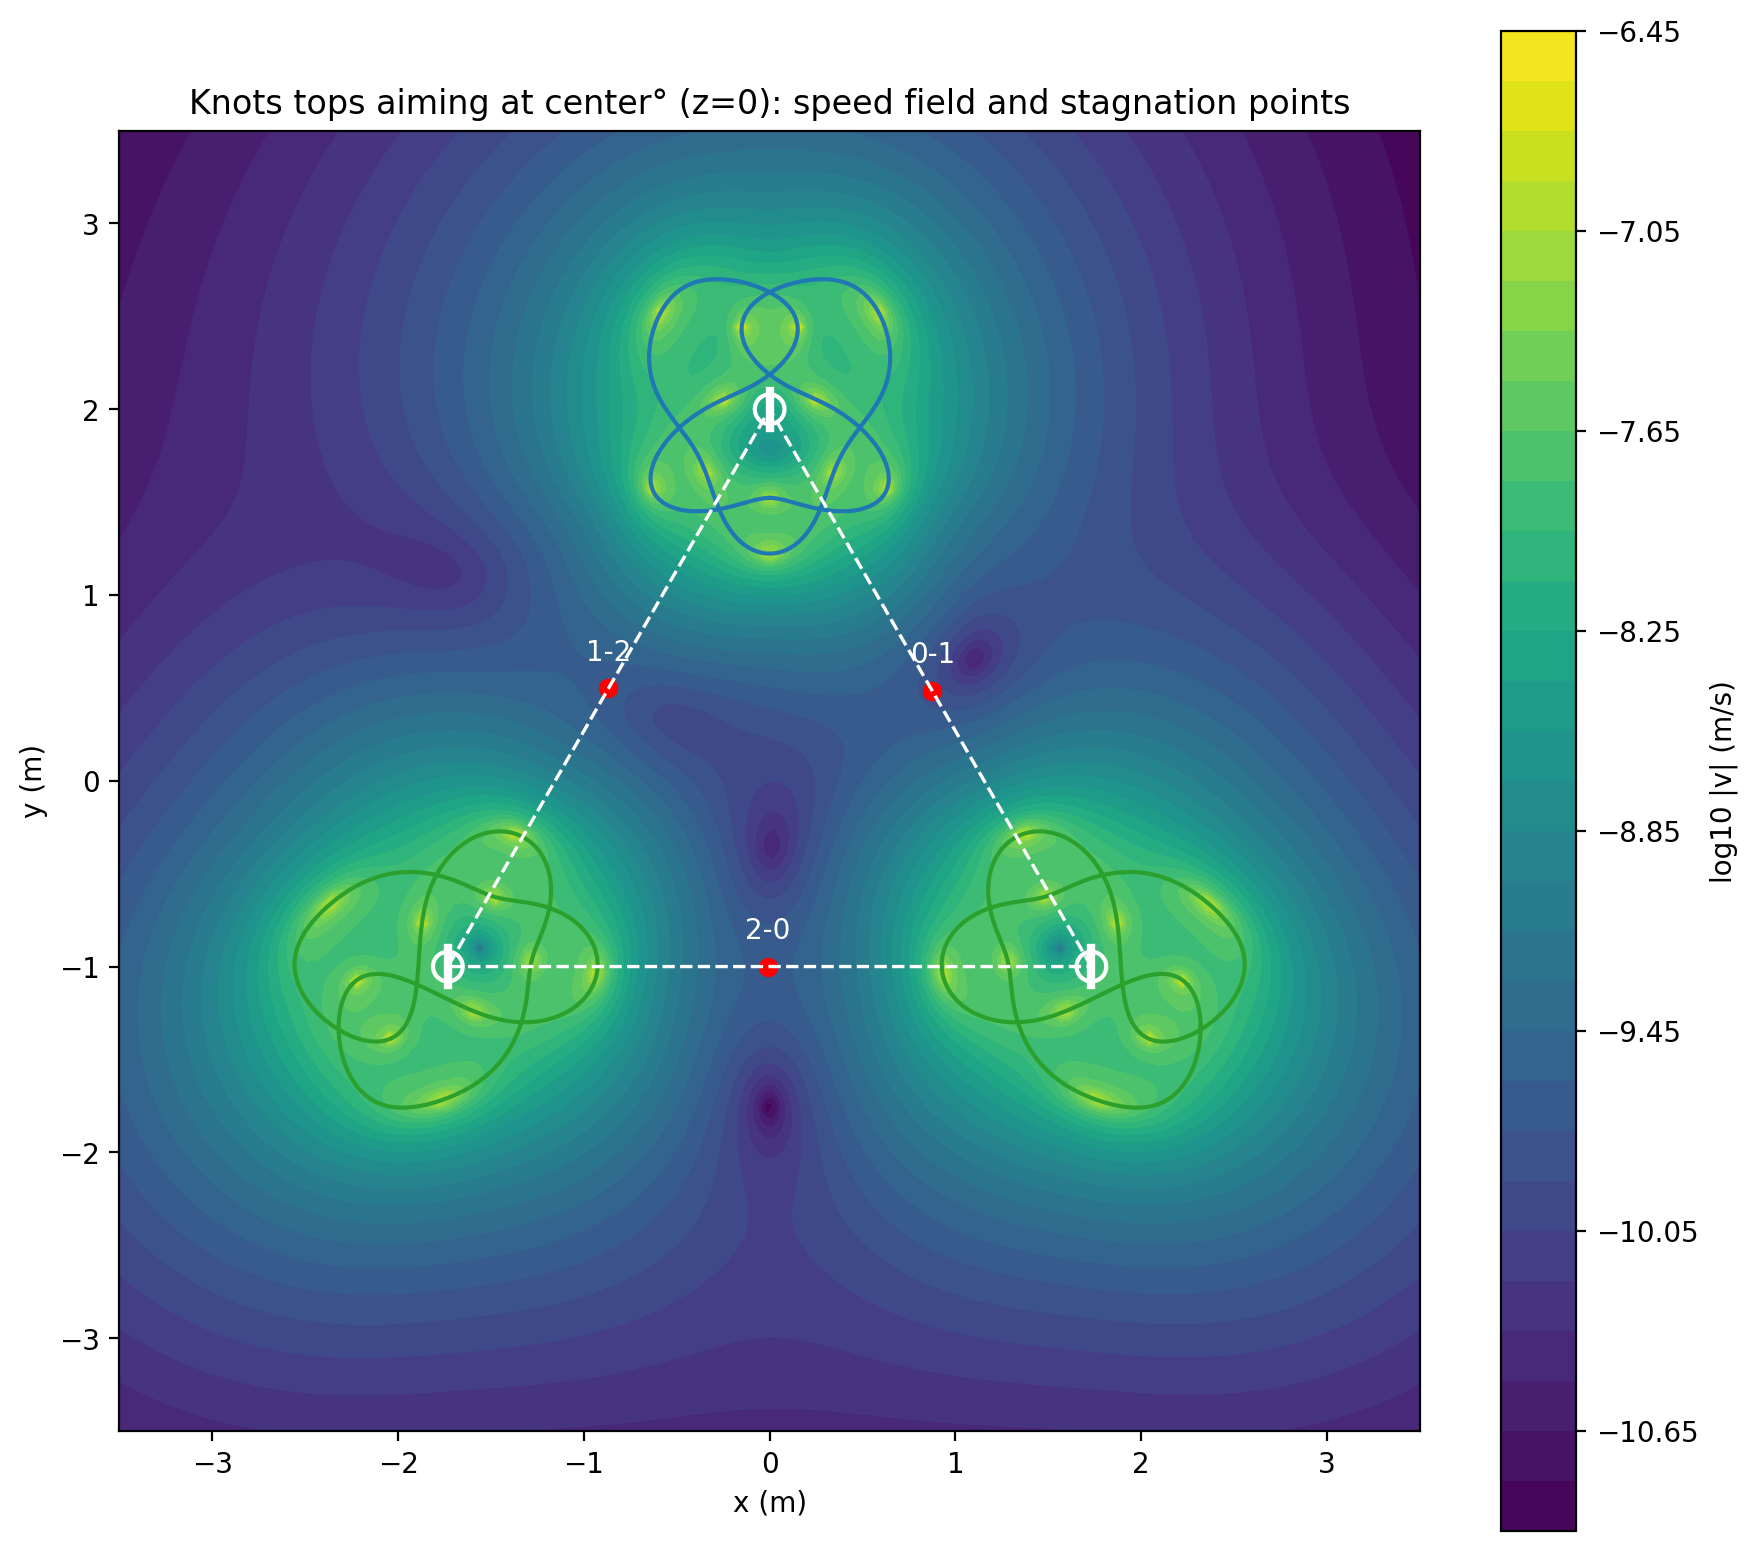
\includegraphics[width=0.3\linewidth]{sst_three_knot_180_speed_stagnation}}
        \subfloat[3D view of 3 quarck knots\label{fig:baryon3d1}]{
            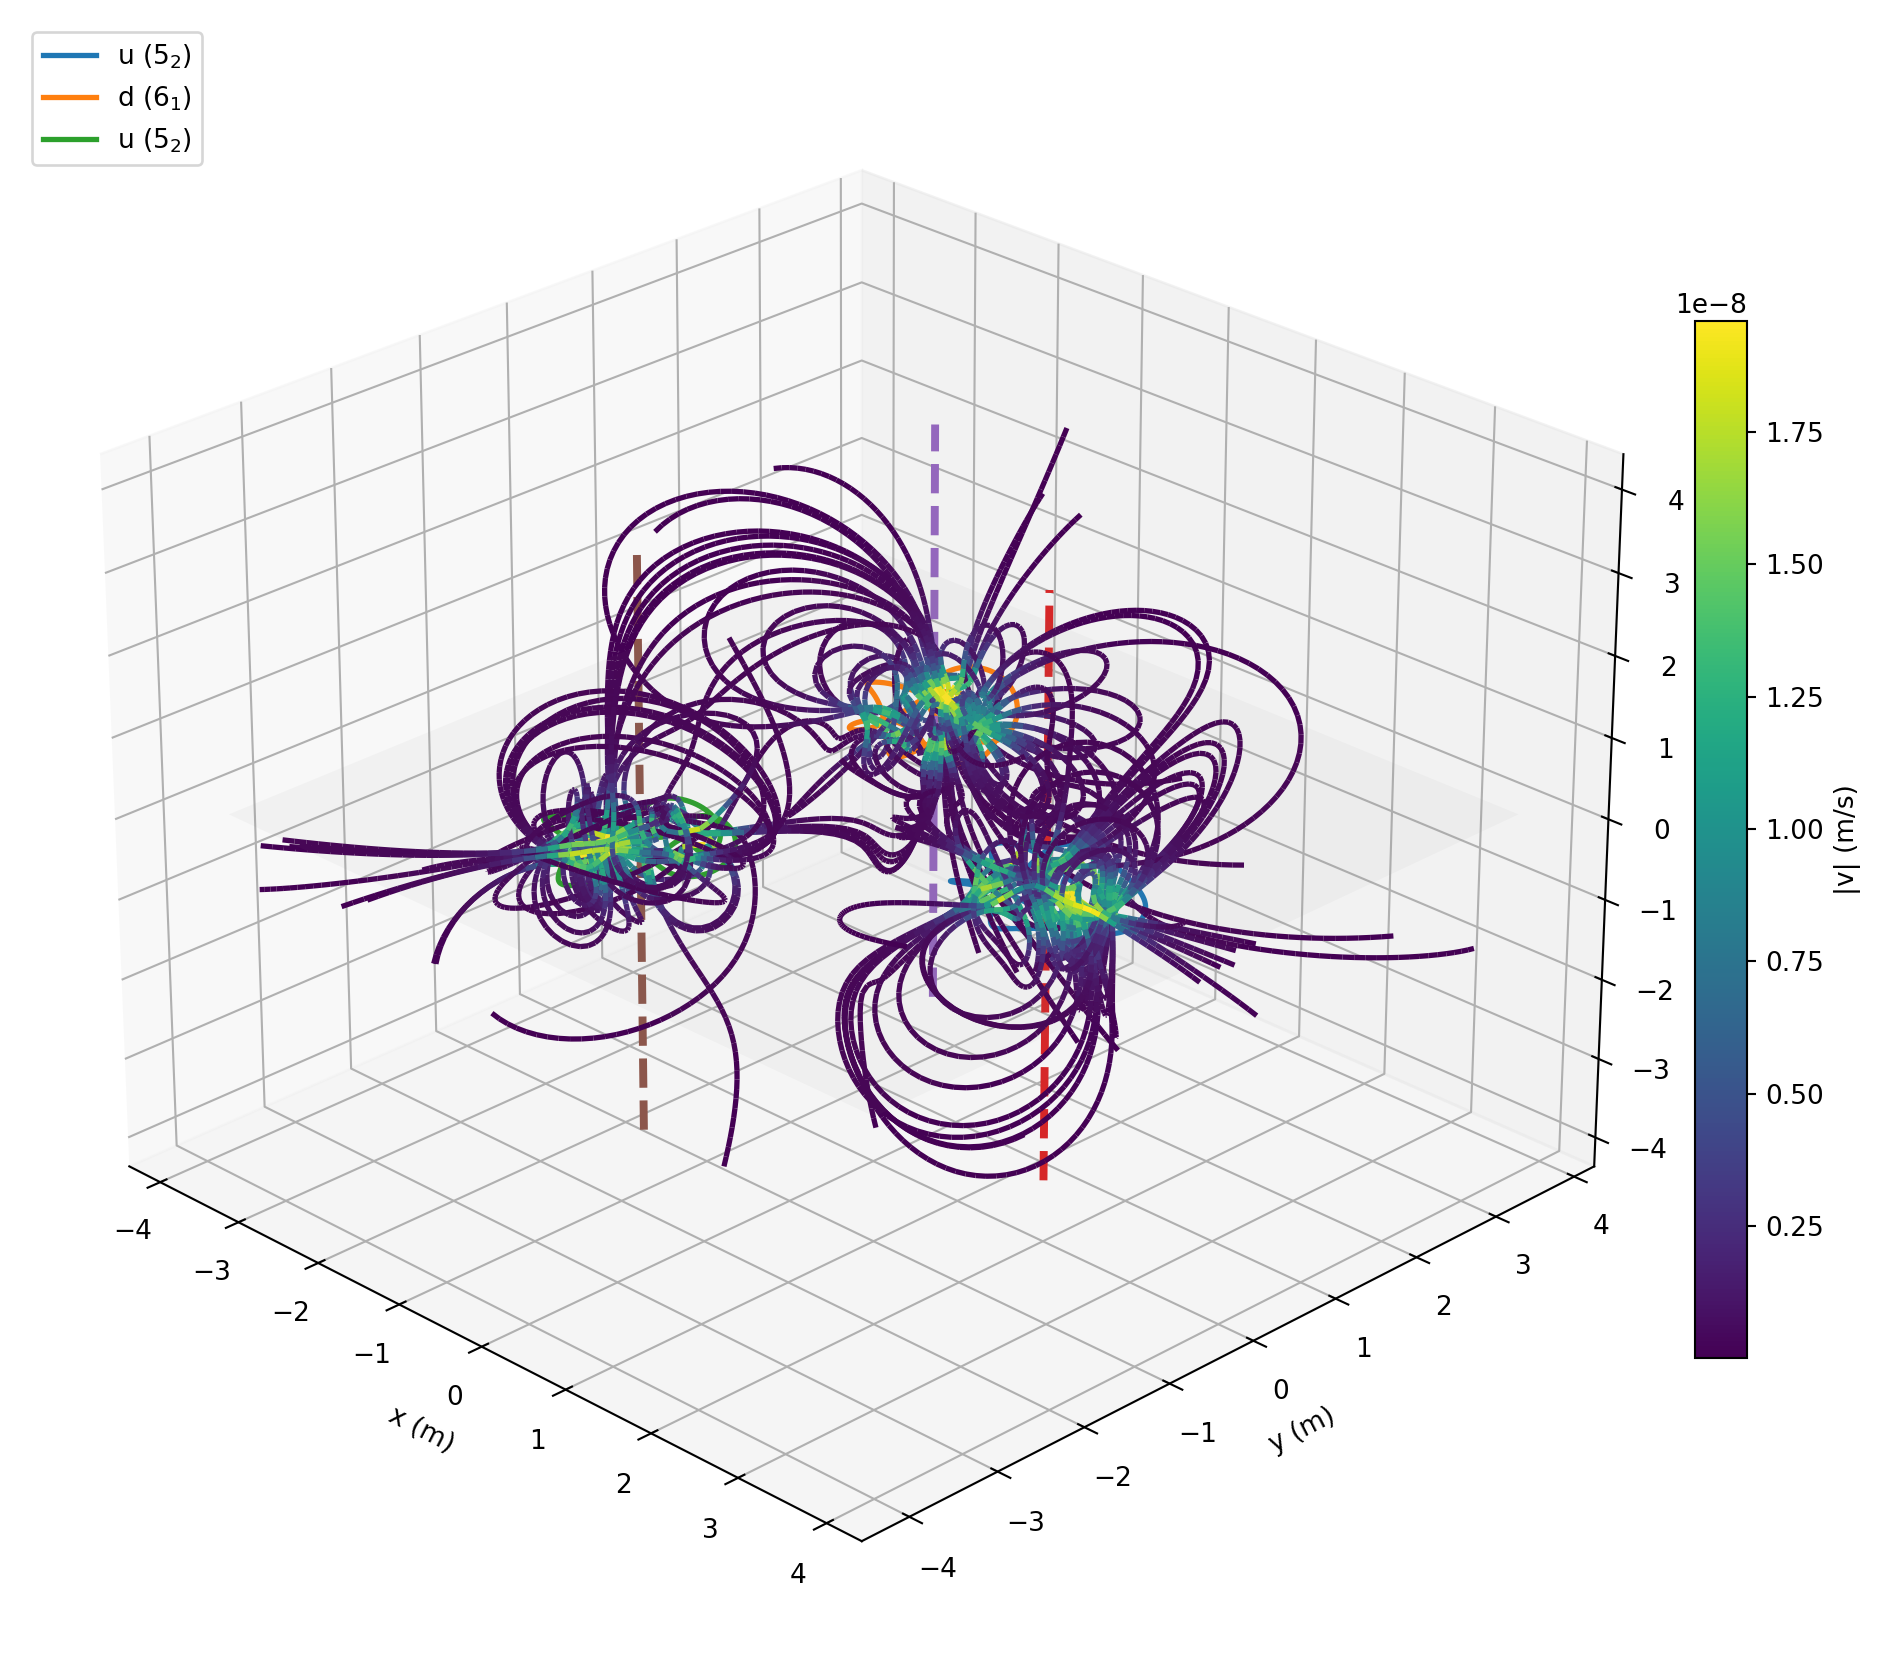
\includegraphics[width=0.3\linewidth]{sst_three_knot_3d_streamlines_colored_ULTRALIGHT}}
        \subfloat[Composite tube\label{fig:baryon_composite_tube}]{

            \begin{tikzpicture}[scale=0.5, line cap=round, line join=round]

                \tikzset{
                    axisline/.style={draw=black!70, line width=0.6pt},
                    tube/.style={draw, line width=2.2pt, rounded corners=2pt},
                    vline/.style={draw, line width=1.2pt},
                    labelbox/.style={fill=white, draw=black!20, rounded corners=2pt, inner sep=3pt}
                }

                \draw[axisline, ->] (0,-5.2) -- (0,4.2) node[left] {$z$};
                \draw[axisline, ->] (-4.2,0) -- (4.2,0) node[below right] {$x$};
                \fill (0,0) circle (2pt);
                \node[below right] at (0,0) {\small central axis};

                % ---------- Three incoming quark tubes (from -z, merging to z-axis) ----------
                \draw[tube, blue!70]
                (-1.8,-5.0) .. controls + (0,2.1) and +(-0.6,-0.3) .. (-0.8,-1.2);
                \draw[tube, green!70!black]
                (0.0,-5.0) .. controls + (0,2.3) and +(-0.2,-0.3) .. (0.0,-1.2);
                \draw[tube, red!70]
                (1.8,-5.0) .. controls + (0,2.1) and +(0.6,-0.3) .. (0.8,-1.2);

                % ---------- Y-junction region into the central tube ----------
                \draw[tube, gray!35] (-0.8,-1.2) -- (-0.25,-0.6);
                \draw[tube, gray!35] ( 0.0,-1.2) -- ( 0.0,-0.6);
                \draw[tube, gray!35] ( 0.8,-1.2) -- ( 0.25,-0.6);

                % ---------- Composite tube along +z on the central axis ----------
                \draw[tube, black!80]
                (0.0,-0.6) .. controls +(0,0.9) and +(0,-0.9) .. (0.0,3.8);

                % ---------- Swirl/flow direction tick marks ----------
                % Incoming (upwards along +z)
                \foreach \x/\z in {-1.5/-4.2, -1.2/-3.2, -1.0/-2.2}{
                    \draw[vline, blue!70] (\x,\z) -- ++(0,0.6);
                }
                \foreach \x/\z in {0.0/-4.4, 0.0/-3.4, 0.0/-2.4}{
                    \draw[vline, green!70!black] (\x,\z) -- ++(0,0.6);
                }
                \foreach \x/\z in {1.5/-4.2, 1.2/-3.2, 1.0/-2.2}{
                    \draw[vline, red!70] (\x,\z) -- ++(0,0.6);
                }
                % Composite (upwards along +z)
                \foreach \z in {-0.2, 0.8, 1.8, 2.8}{
                    \draw[vline, black!80] (0.0,\z) -- ++(0,0.8);
                }

                % ---------- Labels ----------
                \node[align=left, labelbox, anchor=west] at (-3.9,-4.6) {Three quark tubes\\[-2pt]
                    \(\Gamma_1=\Gamma_2=\Gamma_3=\kappa\)};
                \node[align=left, labelbox, anchor=west] at (0.2,2.8) {Composite tube on \(z\)-axis\\[-2pt]
                    \(\Gamma_{\text{baryon}}=3\kappa\)\\[-2pt]
                    \(v_{\theta,\mathrm{eff}}=3\,v_c\)};
                \node[align=left, labelbox, anchor=east] at (-1,-0.2) { \(\ \Gamma=\sum_i \Gamma_i\)};
            \end{tikzpicture}
        }
        \caption{Baryon core as a \emph{composite swirl tube}. Three quark tubes (bottom) join via a Y-junction into a single tube along $+z$. Circulation adds linearly, $\Gamma_{\rm baryon}=3\kappa$, hence $v_{\theta,\rm eff}=\Gamma_{\rm baryon}/(2\pi r_{\rm eff})$ with $r_{\rm eff}\approx r_c$ to leading order.}
        \label{fig:three-knot-gallery}
    \end{figure}

    Each quark knot $i$ has circulation $\Gamma_i = \kappa$ around the central axis (Fig.~\ref{fig:baryon_composite_tube}).
        By Kelvin additivity,
        \begin{equation}
            \Gamma_{\mathrm{baryon}}=\Gamma_1+\Gamma_2+\Gamma_3=3\kappa.
        \end{equation}
        Since $\Gamma=2\pi r\,v_\theta$,
        \begin{equation}
            \boxed{\;
            v_{\theta,\mathrm{eff}}=\frac{\Gamma_{\mathrm{baryon}}}{2\pi\,r_{\mathrm{eff}}}
                =\frac{3\kappa}{2\pi\,r_{\mathrm{eff}}}\,,
                \;}\label{eq:baryon-vtheta}
        \end{equation}
        with $r_{\mathrm{eff}}$ the effective core radius of the merged tube. In the thin-core, near-Rankine limit $r_{\mathrm{eff}}\approx r_c$ to leading order (so that $v_{\theta,\mathrm{eff}}\approx 3 v_c$ holds as a first-order estimate), while the deeper pressure well is set by the increased $\Gamma$.

        \paragraph{Swirl Clock scaling.}
        The Swirl Clock relation becomes
        \begin{equation}
            dt_{\mathrm{local}} = dt_\infty \sqrt{1 - \frac{(3 v_c)^2}{c^2}},\label{eq:baryon-swirl-clock}
        \end{equation}
        predicting a more pronounced local time dilation, consistent with the larger rest mass of baryons relative to single quark knots.

            \emph{Analogy (for intuition).} Three equal water whirls feed one outlet: the hole may widen slightly, but the combined spin deepens the whirl and speeds the rim roughly threefold.





\section{Swirl Gravity and Molecular Attraction}
    Two composite tubes (e.g., two protons) sharing the same central line produce a combined circulation
    \[
        \Gamma_{\mathrm{total}} = (3 \kappa)_{\mathrm{proton}} + (3 \kappa)_{\mathrm{proton}} = 6 \kappa,
    \]
    which deepens the shared pressure well and yields a stronger long-range attraction.
    This explains why neutral molecules (e.g., H$_2$) still attract in Euclidean space: their baryon cores are connected by the same central line, and the resulting swirl gravity follows directly from the additive circulation.

    \subsection{Electromotive Response to Swirl Gravity}

        Recent work in the SST Canon \cite{EMG2025} has demonstrated that time-dependent swirl density \( \partial_t \vec{\rho}_{\circlearrowleft} \) acts as a source term in the modified Faraday law:
        \[
            \nabla \times \vec{E} = -\partial_t \vec{B} - \vec{b}_{\circlearrowleft}, \quad \vec{b}_{\circlearrowleft} = G_{\circlearrowleft} \, \partial_t \vec{\rho}_{\circlearrowleft}
        \]
        Here, \( G_{\circlearrowleft} \) is a universal topological transduction constant, canonically normalized to a flux quantum \( \Phi^\star \in \{ h/e, h/2e \} \). This coupling provides a direct, falsifiable prediction: nucleation or reconnection of vortex lines produces a quantized electromotive impulse of magnitude \( \Phi^\star \). In gravitational contexts, this implies that pressure or density changes which alter swirl topology can be detected electromagnetically. Thus, SST gravity is not only fluid-mechanical but also electromagnetically active — a feature testable in vortex-generating platforms.


    \section{Entropic Embedding of Swirl–String Theory}
\label{sec:entropic-sst}

    Swirl–String Theory (SST), built on topologically quantized circulation in a flat, vortex-supporting medium, lends itself naturally to an entropic reinterpretation. In this section, we demonstrate how SST supports the core principles of Verlinde’s emergent gravity paradigm \cite{verlinde2011origin, verlinde2016emergent}, allowing a consistent embedding of mass, force, and time as information-theoretic quantities.

    \subsection{Swirl Entropy as Informational Field}

        We define a swirl-based entropy field $S_\swirlarrow(x^\mu)$ as a logarithmic function of the swirl areal density $\rho_\swirlarrow = \nabla \cdot \vec{a}$:

        \begin{equation}
            S_\swirlarrow(x^\mu) = k_B \cdot \log\left(1 + \frac{\rho_\swirlarrow(x^\mu)}{\rho_0}\right)
        \end{equation}

        Here, $\rho_0$ is a constant baseline density. The field $S_\swirlarrow$ plays the role of local entropy density, similar to that on a holographic screen in entropic gravity.

    \subsection{Entropic Force from Swirl Gradients}

        Verlinde’s entropic force expression is:

        \begin{equation}
            F = T \cdot \frac{dS}{dx}
        \end{equation}

        In SST, circulation-induced pressure deficits are given by:

        \begin{equation}
            \Delta p = -\frac{1}{2} \rho_f v^2
        \end{equation}

        Assuming that swirl flow aligns with entropy gradient, the effective force becomes:

        \begin{equation}
            F_\text{swirl} \propto \nabla \rho_f v^2 \propto \nabla S_\swirlarrow
        \end{equation}

        This establishes a direct analogy between entropic forces and swirl-induced attractions in SST.

    \subsection{Mass as Topological Information}

        In SST, mass is given by the circulation quantum $\kappa$:

        \begin{equation}
            m = \frac{h}{\kappa}, \qquad \kappa = 2\pi r_c v_c
        \end{equation}

        Interpreting $\kappa$ as a unit of quantized topological information, mass becomes a discrete sum over informational elements:

        \begin{equation}
            m_K = \sum_i \epsilon_i, \quad \epsilon_i = \frac{h}{\kappa_i}
        \end{equation}

        This matches Verlinde’s picture of mass as emergent from underlying information content.

    \subsection{Time Dilation as an Entropic Clock}

        SST defines a Swirl Clock for local proper time as:

        \begin{equation}
            dt_\text{local} = dt_\infty \sqrt{1 - \frac{v^2}{c^2}}
        \end{equation}

        This behavior is consistent with entropic gravity, where time slows in regions of higher information density, i.e., higher $\rho_\swirlarrow$.

    \subsection{R/T Phase Transition and Information Localization}

        SST posits two phases:
        \begin{itemize}
        \item \textbf{R-phase}: unknotted, wave-like field state
        \item \textbf{T-phase}: knotted, particle-like topological excitation
        \end{itemize}

        The R-to-T transition represents an entropic localization, akin to wavefunction collapse and entanglement decoherence. This dynamic aligns SST with entropy-based emergence of space and matter.

    \subsection{Summary of Mapping}

        \begin{table}[h]
            \centering
            \begin{tabular}{lll}
                \toprule
                \textbf{SST Concept} & \textbf{Entropic Gravity Analog} & \textbf{Interpretation} \\
                \midrule
                $\rho_\swirlarrow$ & Entropy density & Local information field \\
                Swirl clock & Gravitational redshift & Entropic time rate \\
                $\Delta p$ & Entropic force & Gradient of entropy \\
                $\kappa$ & Info unit / bit & Mass from information \\
                R/T transition & Wave collapse & Information localization \\
                \bottomrule
            \end{tabular}
            \caption{Correspondences between SST and Verlinde's entropic gravity.}\label{tab:sst-entropic-mapping}
        \end{table}

        SST, therefore, may be interpreted as an entropic field theory in flat space, where gravitational and inertial phenomena arise from topological and informational structures.

    \section{Lagrangian and Action Formulation}

        The dynamical content of Swirl–String Theory (SST) can be expressed via an effective Lagrangian density \( \mathcal{L} \) over a flat spacetime manifold, with swirl fields defined by a scalar potential \( \phi(x^\mu) \), a swirl vector potential \( a_\mu(x^\nu) \), and a fluid mass density field \( \rho_f \). The swirl areal density is defined as \( \rho_\circ = \nabla \cdot \vec{a} \). The field strength tensor is analogous to Maxwell's:
        \[
            F_{\mu\nu} = \partial_\mu a_\nu - \partial_\nu a_\mu
        \]
        The full Lagrangian density is:
        \[
            \mathcal{L}_{\text{SST}} = -\frac{1}{4} F_{\mu\nu} F^{\mu\nu} + \rho_f \, (\partial_\mu \phi)(\partial^\mu \phi) - V(\phi) + \mathcal{L}_\text{topo}
        \]
        where \( V(\phi) \) encodes the knot potential and \( \mathcal{L}_\text{topo} \) captures topological coupling terms from knot genus and braid index.

        The action is then:
        \[
            S = \int \mathcal{L}_{\text{SST}} \, d^4x
        \]
        Euler–Lagrange equations derived from this action yield conservation laws and field dynamics for both swirl flow and entropic gravity analogs.

        In the case of hydrogenic systems, swirl gradients around knot cores induce pressure deficits which couple directly to particle motion via Bernoulli and Euler field dynamics — reproducing effective gravitational behavior without spacetime curvature.


    \emph{If the SST swirl core modulates local time dilation, then ultra-precise molecular spectroscopy (e.g., of H₂ or H₃⁺ ions) could detect deviations correlated with topological configurations, offering an experimental test of the Swirl Clock hypothesis.}


        "The quantized vortex mass formula, derivation of the swirl Schrödinger equation, and finite-core energy regularization were previously established in the VAM framework [Iskandarani, 2024]. The present work translates and updates these within the SST notation via the Rosetta map [Iskandarani, 2025]."

        \mathcal{L}_\text{SST} = -\frac{1}{4} F_{\mu\nu} F^{\mu\nu} + \rho_f (\partial_\mu \phi)(\partial^\mu \phi) - V(\phi)

    \section{Legacy Foundations and Rosetta Translation}
    \label{sec:legacy-rosetta}

        The formal structure of Swirl–String Theory (SST) builds upon a previously established framework of topological fluid dynamics developed in the Vortex–Æther Model (VAM). This legacy model derived key physical results from circulation quantization and fluid field dynamics, including a topologically quantized mass formula, a swirl-based Schrödinger equation, and a non-divergent fluid Lagrangian. These results have been translated and reformulated within SST via a symbolic mapping documented in the Rosetta file \cite{vamrosetta2025}.

    \subsection{Quantized Circulation and Mass Formula}

        In VAM, the core mass mechanism arises from Onsager-like circulation quantization:
        \begin{equation}
        \oint \vec{v} \cdot d\vec{\ell} = n \kappa_\text{æ}
        \end{equation}
        with velocity expressed as a gradient:
        \begin{equation}
        \vec{v} = \lambda_\text{æ} \nabla \theta \quad \Rightarrow \quad \psi = \sqrt{\rho/\rho_\text{æ}}\, e^{i\theta}
        \end{equation}
        leading to a hydrodynamic Schrödinger equation with swirl potential:
        \begin{equation}
        i\hbar_\text{æ} \frac{\partial \psi}{\partial t} = -\frac{\hbar_\text{æ}^2}{2m_\text{æ}} \nabla^2 \psi + \Phi_{\text{swirl}}(\vec{\omega})\, \psi
        \end{equation}
        \begin{equation}
        \Phi_{\text{swirl}} = \frac{1}{2} \lambda_g \rho_\text{æ} |\vec{\omega}|^2
        \end{equation}
        This formulation yielded vortex mass estimates (e.g. for the electron) within \( <10^{-7} \) error of experimental values.

    \subsection{Lagrangian and Field Formalism}

        VAM also provided a fluid Lagrangian consistent with gauge-invariant dynamics:
        \begin{equation}
        \mathcal{L}_\text{VAM} = \frac{1}{2} \rho_f (\nabla \times \vec{A})^2 + \rho_f (\partial_t \phi)^2 - V(\phi)
        \end{equation}
        This maps directly into the SST flat-space field theory:
        \begin{equation}
        \mathcal{L}_\text{SST} = -\frac{1}{4} F_{\mu\nu} F^{\mu\nu} + \rho_f (\partial_\mu \phi)(\partial^\mu \phi) - V(\phi) + \mathcal{L}_{\text{topo}}
        \end{equation}
        where the swirl vector \( a_\mu \) replaces the VAM circulation potential, and \( \mathcal{L}_{\text{topo}} \) incorporates topological invariants (braid index, genus, component count).

    \subsection{Notation Fidelity via Rosetta Map}

        All constants, fields, and structural equations have been translated via the VAM–SST Rosetta dictionary \cite{vamrosetta2025}, ensuring full dimensional and symbolic consistency. This includes:
        \begin{itemize}
        \item Swirl velocity: \( \vec{v}_{\circlearrowleft} = \nabla \phi \)
        \item Core swirl speed: \( \|\vec{v}_{\circlearrowleft}\| = 1.093 \times 10^6\ \text{m/s} \)
        \item Core radius: \( r_c = 1.40897 \times 10^{-15}\ \text{m} \)
        \item Core density: \( \rho_{\text{core}} = 3.89 \times 10^{18}\ \text{kg/m}^3 \)
        \item Time variables: external time \( \tau \), swirl clock \( S(t) \), and proper loop time \( T_s \)
        \end{itemize}

        This lineage confirms that SST inherits a fully variational, quantized, and empirically calibrated foundation — now recast in a swirl-theoretic, flat-space field formalism.



    \section{Conclusion}
        Long-distance gravitational attraction in SST is a manifestation of topological quantization: chiral knots with central holes enforce non-vanishing circulation residues along a central line.
        When multiple quark knots merge into a baryon, their circulations add linearly, forming a single composite tube with $3\kappa$ circulation.
        This mechanism predicts the correct baryonic mass scaling and provides a flat-space explanation for molecular attraction.

    \section*{Code and Data Availability}
        All predictive simulations used in this paper are implemented in the open Python script \texttt{SST\_INVARIANT\_MASS3.py}, available on request or at Zenodo: \url{https://doi.org/10.5281/zenodo.17155854}


\nocite{*}
\bibliographystyle{unsrt}
\bibliography{swirlgravity}






\end{document}
